\item For a given vector $\vec{w} = \myvec{ 1 \\ 2 \\ 3 }$, the vector normal to the plane defined by $\vec{w}^T \vec{x} = 1$ is \hfill{(EE 2023)}
\begin{multicols}{4}
\begin{enumerate}
    \item $\myvec{ -2 \\ -2 \\ 2 }$
    \item $\myvec{ 3 \\ 0 \\ -1 }$
    \item $\myvec{ 3 \\ 2 \\ 1 }$
    \item $\myvec{ 1 \\ 2 \\ 3 }$
\end{enumerate}
\end{multicols}
\item In the figure, the vectors $\vec{u}$ and $\vec{v}$ are related as $\vec{A}\vec{u} = \vec{v}$ by a transformation matrix $\vec{A}$. The correct choice of $\vec{A}$ is \hfill{(EE 2023)}
\begin{figure}[H]
    \centering
    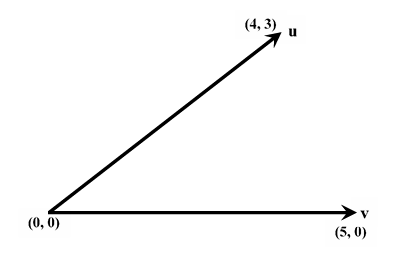
\includegraphics[width=0.5\columnwidth]{GATE/2023/EE/figs/Q 24.png}
    \caption{}
    \label{fig:placeholder/2023/33}
\end{figure}
\begin{multicols}{4}
\begin{enumerate}
    \item $ \myvec{
\dfrac{4}{5} & \dfrac{3}{5} \\
\dfrac{3}{5} & -\dfrac{4}{5}
}$
    \item $ \myvec{
\dfrac{4}{5} & -\dfrac{3}{5} \\
\dfrac{3}{5} & \dfrac{4}{5}
}$
    \item $ \myvec{
\dfrac{4}{5} & \dfrac{3}{5} \\
\dfrac{3}{5} & \dfrac{4}{5}
}$
    \item $ \myvec{
\dfrac{4}{5} & -\dfrac{3}{5} \\
\dfrac{3}{5} & -\dfrac{4}{5}
}$
\end{enumerate}
\end{multicols}
\item Three points in the $x$-$y$ plane are $(-1,~0.8), (0,~2.2)$ and $(1,~2.8)$. The value of the slope of the best fit straight line in the least square sense is \rule{2cm}{0.15mm}. 

	\hfill{(EE 2023)}
\item Consider the following equation in a 2-D real-space.
$$
|x_1|^p + |x_2|^p = 1 \quad \text{for } p > 0
$$
Which of the following statement(s) is/are true.\hfill{(EE 2023)}
\begin{enumerate}
    \item When $p=2$, the area enclosed by the curve is $\pi$.
    \item When $p$ tends to $\infty$, the area enclosed by the curve tends to $4$.
    \item When $p$ tends to $0$, the area enclosed by the curve is $1$.
    \item When $p=1$, the area enclosed by the curve is $2$.
\end{enumerate}
\item A quadratic function of two variables is given as
$$
f(x_1, x_2) = x_1^2 + 2x_2^2 + 3x_1 + 3x_2 + x_1 x_2 + 1
$$
The magnitude of the maximum rate of change of the function at the point $(1,1)$ is \underline{\hspace{2.5cm}}. \hfill{(EE 2023)}

